\chapter{Backend}

Moderní webové aplikace lze rozdělit na back a frontend. Backend je část aplikace, která běží na serveru. Pomocí svých služeb poskytuje přístup k databázi, k souborům uloženým na serveru a zpracovává uživatelské operace. Frontend těchto služeb využívá. Tato kapitola popisuje proces výběru backendových technologií pro tuto práci. Některé technologie se osvědčily, jiné se ukázaly pro daný účel nevhodné.

\section{Databáze}

Úkolem databáze je uložit data a umožnit jejich prohledávání. Důležitou vlastností naší aplikace je, že uživatelé nemají možnost databázi modifikovat. Zápis do databáze provede administrátor pouze jednou, před startem aplikace. Důležitým požadavkem je důraz na rychlost a snadnou škálovatelnost. V posledních letech vzniklo několik nových databází v kategorii vágně označené jako NoSQL\cite{nosql}. Tato kategorie databází se těžko popisuje, na každou popsanou vlastnost existuje NoSQL databáze, která danou vlastnost nesplňuje. Obecně ale lze říct že NoSQL databáze nepracují s prvky v tabulkovém uspořádání a oproti standardním SQL databázím nekladou tolik omezujících požadavků na data. Jejich výhodou oproti standardním relačním databázím může být vyšší výkon a snadná škálovatelnost.

Nevýhodou je většinou obtížnější práce s daty. Většina NoSQL databází například mapodporuje databázové transakce a vůbec celý ACID. Pro práci s daty v NoSQL databázi nelze použít klasické SQL dotazy. Místo nich se používá například model MapReduce\cite{mapreduce} vyvinutý ve formě Google.

První verze aplikace byla postavena na databázi CouchBase\cite{couchbase}, což je právě jedna z NoSQL databází podporující MapReduce mechanismus. Výhodou CouchBase je vysoký výkon, snadná škalovatelnost, velmi dobrá dokumentace a také existence oficiálních knihoven pro nejrozšířenější programovací jazyky. Ukázalo se však, že pro implementaci vyhledávání pro naší aplikaci je model MapReduce nedostatečný a implementace vyhledávání v CouchBase by byla prakticky nemožná.

Vhodnější pro daný účel se ukázala knihovna Elasticsearch\cite{elasticsearch}. Nejedná se v pravém smyslu o databázi. Jejím hlavním cílem je poskytnout vyhledávání nad daty. Je postavená nad knihovnou Apache Lucene ke které přidává snadnou horizontální i vertikální škálovatelnost a komunikaci pomocí REST HTTP JSON API. Díky tomu, že je Elasticsearch postaven na knihovně Lucene\cite{lucene}, může programátor využít velkou množinu možností, které Lucene poskytuje. Například v  textovém vyhledávání může využít všechny tokenizery a stemmery z knihovny Lucene. V průběhu implementace aplikace navíc vyšla stabilní verze 1.0.

\section{Programovací jazyk}

Volba programovacího jazyka je při tvorbě backendové části klíčová. Tato sekce rozebírá některé výhody a nevýhody třech programovacích jazyků.

\subsection{NodeJS}

JavaScript je jazyk především pro programování frontendu a dlouho byl brán jako nutné zlo --- bez použití problematických rozšíření nejde ve webovém prohlížeči programovat jiným jazykem. Každý větší webový projekt tak byl nucen používat nejméně 2 technologie --- jednu pro frontend a jednu pro backend. Knihovna NodeJS toto paradigma obrací, umožňuje programovat v JavaScriptu i na backendu. Výhodou je sdílení stejného kódu mezi backendem a frontendem. To se hodí například při validacích dat, které potřebujeme kontrolovat na frontendu i backendu.

Původní záměr byl využít pro vývoj naší aplikace právě NodeJS. Nakonec však převážily nevýhody takového řešení.Javascript byl navržen pro programování webového frontendu, jeho standartní knihovna je v porovnání s ostatními jazyky velmi chudá, podpora objektového programování není přímočará. Obsáhlý kód v Javascriptu může být poměrně nepřehledný a jazyk svádí k vytvoření takzvaného \uv{callback hell}. Ukázka takového problémového kódu je v článku \cite{callback}

\begin{lstlisting}
doAsync1(function () {
  doAsync2(function () {
    doAsync3(function () {
      doAsync4(function () {
    })
  })
})
\end{lstlisting}


 Pokud chce navíc programátor sdílet kód z backendu i na frontendu, musí být kód kompatibilní s podporovanými prohlížeči. Pokud aplikace potřebuje podporovat starší verze prohlížečů, nemůže sdílený kód obsahovat novinky z páté verze ECMAScript\cite{ecma}.

\subsection{Go}

Go (známý také jako golang)\cite{golang} je staticky typovaný programovací jazyk od společnosti Google. Syntaxe je inspirována jazykem C s důrazem rychlou kompilaci. Velkou výhodou je snadná práce s vlákny pomocí \uv{goroutines}. Programátoři v Javě, nebo C++ může překvapit poněkud netypická podpora práce s objekty.

První verze aplikace byla napsána právě v jazyce Go. Později byla přepsána většina v jazyce Ruby. Výhodou řešení v jazyce Go je velká výkonost a stabilita aplikace. Zkompilovaná aplikace je pouze jeden binární soubor, takže oproti řešení v nekompilovaných jazycích se lépe distribuuje a odpadají problémy se závislostmi.

Go je stále poměrně mladý jazyk, první stabilní byla vydána teprve v roce 2012\cite{golang-release}. Největším problémem takto mladých jazyků je nedostatek kvalitních knihoven. Pokud už na daný problém existuje knihovna, těžko se odhaduje, jestli její autor projekt neopustí a jestli bude knihovna podporována i další rok. Pro naší aplikaci se ukázal jako problém neexistence kvalitní knihovny pro komunikaci s databází Elasticsearch. S tou jde komunikovat pomocí HTTP requestů, takže jsme pro naší potřebu vytvořili jakousi mikroknihovnu. Experimentální povaha aplikace ovšem vyžadovala rychlé prototypování a úprava kódu na komunikaci s Elasticsearch začala být příliš omezující. Pro naše účely se ukázalo výhodnější přepsat hlavní část aplikace do dynamického jazyka s lepší podporou pro Elasticsearch.

V jazyce Go je napsána nezávislá komponenta vyhledávání podobných obrázků, která je popsána v Kapitole \ref{chap:similar}.

\subsection{Ruby a Ruby on Rails}

Ruby\cite{ruby} je dynamicky typovaný jazyk, inspirovaný jazyky jako Perl, nebo Smalltalk, s důslednou podporou objektového programování. Popularita Ruby vzrostla zejména díky webovému frameworku Ruby on Rails (Rails)\cite{rails}, který je v Ruby napsaný. Rails zpopularizovaly architekturu Model-View-Controller\cite{mvc} pro tvoru webových aplikací. Backend aplikace s vyjímkou služby pro vyhledávání podobných obrázků, byl nakonec přepsán právě do Rails. Elasticsearch poskytuje pro práci s Ruby oficiálně podporovanou knihovnu\cite{elasticsearch-ruby}. Další výhodou se knihovna Rake, což je obdoba příkazu Make pro skripty v Ruby. Pomocí Rakefilu jdou napsat přehledné úlohy pro manipulaci s daty. 

\section{Komunikace mezi backendem a frontendem}

Tato sekce popisuje možnosti komunikace mezi frontendem a backendem.

\subsection{Formát dat}

Nejprve je potřeba zvolit formát dat. V součastnosti existují dva nejrozšířenější textové komunikační formáty --- XML\cite{xml} a JSON\cite{json}. XML umožňuje popis velkého množství vztahů mezi entitami. JSON je oproti XML úspornější. XML se hodí v případech, kdy potřebujeme zaznamenat nějaké složité datové struktury. Pro většinu webových aplikací je výhodnější použít JSON. Oproti XML je zápis dat v JSON většinou kratší, což je výhodné zejména při přenosu dat po síti. JSON je založen na datových typech JavaScriptu a moderní prohlížeče umí tento formát zpracovávat nativně. Na frontendu je tedy práce s JSON oproti  práci s XML jednodušší. Z těchto důvodů poskytuje backend naší aplikace služby frontendu ve formátu JSON.

\subsection{REST API}

Dále je potřeba specifikovat způsob výměny dat. Jednou z nejrozšířenějších metod je REST, zkratka pro anglické \uv{Representational state transfer}. Jedná se o architekturu rozhraní mezi klientem a serverem. Pro specifikaci rozhraní využívá protokol HTTP. REST využívá k definici práce s daty metody protokolu HTTP \uv{GET}, \uv{PUT}, \uv{POST} a \uv{DELETE}.

Rozhraní REST\cite{rest} s použitím formátu JSON je v aplikaci využíváno pro komunikaci s databází Elasticsearch i pro komunikaci mezi backendem a frontendem.

\subsection{WebSocket}

\begin{figure}[h]
  \centering
  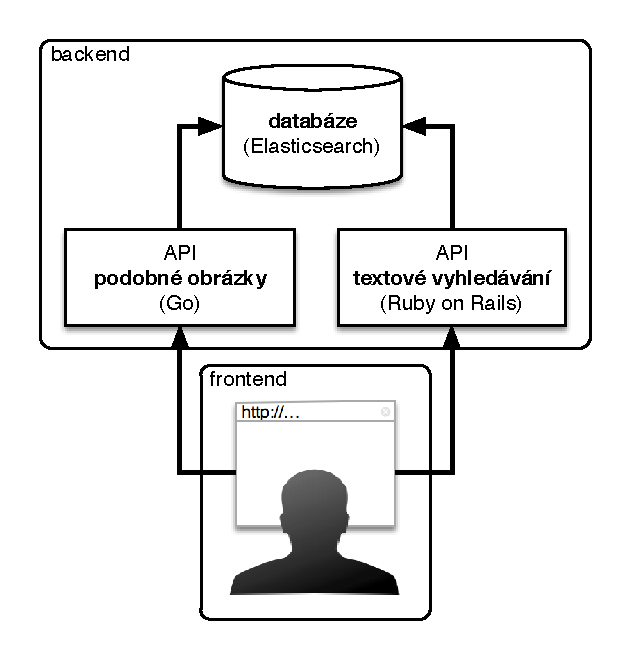
\includegraphics[width=80mm]{architecture.eps}
  \caption{Architektura aplikace.}
  \label{fig:architecture}
\end{figure}

Alternativou k REST API a protokolu HTTP je protokol WebSocket\cite{websocket}. WebSocket je stejně jako protokol HTTP postaven nad protokolem TCP. Na rozdíl od HTTP ale poskytuje duplexní spojení. Klient je tedy stále spojený se serverem a oba mohou posílat zprávy bez ohledu na druhou stranu. Spojení přes WebSocket má většinou menší latenci než použití protokolu HTTP\cite{websocket-study}. Protokol je podporován všemi moderními verzemi webových prohlížečů a podpora existuje i v knihovnách pro backendové programovací jazyky.

První verze aplikace používali pro komunikaci mezi klientem a serverem právě protokol WebSocket. Nakonec však převážily nevýhody takovéhoto řešení nad výhodami. Jednou z nevýhod je nutnost udržovat spojení s klientem na serverové i klientské straně. Přináší to několik netriviálních technických problémů. Například v okamžik, kdy se toto spojení přeruší. Pokud se naproti tomu přeruší spojení server-klient při HTTP požadavku, může klient zkusit vyslat stejný požadavek znovu.

Druhým problémem je emulace HTTP požadavků v protokolu WebSocket. Z klienta můžeme odeslat HTTP dotaz na server a dostaneme k němu přiřazenou odpověď. V protokolu WebSocket pošleme serveru zprávu a za nějaký čas můžeme dostat zprávu od serveru jako odpověď. Párování došlých zpráv z odeslanými zprávami --- požadavky --- ale musíme implementovat sami, například pomocí unikátních identifikátorů v těle zprávy. Naše implementace navíc musí umět řešit situaci, kdy žádná odpověď ze serveru nedojde. Například nastavením timeoutu pro čekání na odpověď.

Řešení pomocí protokolu WebSocket využijí zejména aplikace, které potřebují komunikovat obousměrně mezi klientem a serverem, nebo je pro ně důležitá nízká latence získání odpovědi. Takovými aplikacemi mohou být chatovací služby, nebo online hry. Pro většinu ostatních aplikací budou zatím spíše převažovat nevýhody obtížnějšího technického řešení nad přínosy technologie WebSockets.

\section{Shrnutí}


Architektura je zobrazena na obrázku \ref{fig:architecture}. Část aplikace, která se stará extrakci klíčových slov a textové vyhledávání obrázků je napsána v jazyce Ruby a frameworku Ruby on Rails. Frontend dále komunikuje se službou pro vyhledávání podobných obrázků, která je napsána v jazyce Go. Data jsou uložená v databázi Elasticsearch. Komunikace mezi všemi komponentami probíhá pomocí HTTP REST API, data jsou přenášena ve formátu JSON.








